\documentclass[a4paper, 11pt]{book}
\usepackage[utf8]{inputenc}
\usepackage[T1]{fontenc}

\usepackage[margin=1in]{geometry}
\usepackage{amsmath, amsfonts, amsthm, amssymb, amsxtra}

\usepackage{graphicx}
\usepackage{float}

\usepackage[portuguese]{babel}

\usepackage[dvipsnames]{xcolor}

\usepackage{cmbright}

\usepackage{tabularray}
\usepackage{enumitem}
\usepackage{multicol}

\usepackage{caption} 
\captionsetup{justification=centering} 

\usepackage{hyperref}
\hypersetup{hidelinks}

\usepackage{tikz}
\usetikzlibrary{intersections, angles, calc, positioning}
\usetikzlibrary{shapes.geometric, arrows.meta}
\usetikzlibrary{decorations.pathmorphing, decorations.pathreplacing}

\usepackage[explicit]{titlesec}
\usepackage[letterspace=100]{microtype}
\usepackage{fmtcount}

\titleformat{\chapter}[display]
{\bfseries\large\sf\lsstyle}
{\huge\filleft\mbox{\MakeUppercase{\chaptertitlename} \NUMBERstring{chapter}}}
{1.5ex}
{\titlerule
\vspace*{1.1ex}%
\MakeUppercase{#1}}
[\vspace*{1.5ex}%
\titlerule]
\titlespacing*{\chapter}{0pt}{-10pt}{25pt}

\titleformat{\section}{\Large\bfseries\sffamily\centering}{\thesection}{0.5em}{#1}

\usepackage{thmtools}
\usepackage{thm-restate}
\usepackage[framemethod=TikZ]{mdframed}
\mdfsetup{skipabove=1em,skipbelow=0em, 
innertopmargin=9pt, innerbottommargin=8pt,
innerleftmargin=8pt, innerrightmargin=8pt}

\renewcommand{\qedsymbol}{$\Box$}

\theoremstyle{definition}

\declaretheoremstyle[headfont=\bfseries\sffamily, bodyfont=\normalfont, mdframed={nobreak}]{thmbox}
\declaretheorem[style=thmbox, name=Definição, numberwithin=chapter]{dbox}
\declaretheorem[style=thmbox, name=Teorema, numberwithin=chapter, sibling=dbox]{tbox}
\declaretheorem[style=thmbox, name=Proposição, numberwithin=chapter, sibling=dbox]{pbox}
\declaretheorem[style=thmbox, name=Corolário, numberwithin=chapter, sibling=dbox]{cbox}
\declaretheorem[style=thmbox, name=Lema, numberwithin=chapter, sibling=dbox]{lbox}

\declaretheoremstyle[headfont=\bfseries\sffamily, bodyfont=\normalfont]{exp}
\declaretheorem[style=exp, name=Exemplo, numberwithin=chapter, sibling=dbox]{ex}

\declaretheoremstyle[headfont=\sffamily\itshape, bodyfont=\normalfont]{pr}
\declaretheorem[numbered=no, style=pr, name=Demonstração, qed=\qedsymbol]{prf}

\newcommand{\obs}{\noindent{\textbf{\textcolor{black}{\sffamily Observação:}}}~}

\setlength{\parskip}{5pt}

\newcommand{\medcup}{\mathsf{U}}

\newcommand{\bN}{\mathbb{N}}
\newcommand{\bZ}{\mathbb{Z}}
\newcommand{\bQ}{\mathbb{Q}}
\newcommand{\bR}{\mathbb{R}}
\newcommand{\bC}{\mathbb{C}}
\newcommand{\bK}{\mathbb{K}}

\newcommand{\bz}{\mathbf{0}}

\newcommand{\cA}{\mathcal{A}}
\newcommand{\cB}{\mathcal{B}}
\newcommand{\cC}{\mathcal{C}}
\newcommand{\cM}{\mathcal{M}}
\newcommand{\cL}{\mathcal{L}}
\newcommand{\cP}{\mathcal{P}}

\newcommand{\NN}[1]{\left\Vert #1 \right\Vert}

\usepackage{csquotes}
\usepackage[backend=biber, maxbibnames=5, minbibnames=3, sorting=none, url=false, isbn=false, doi=false, defernumbers=true]{biblatex}
\addbibresource{bibliography.bib}


\begin{document}

\tableofcontents

\addcontentsline{toc}{chapter}{Lista de Símbolos}
\chapter*{Lista de Símbolos}
\begin{tblr}{
    colspec={ll},
    column{1} = {leftsep=0pt, rightsep=15pt}
    }
    $\cB$               & Álgebra de Borel\\
    $\chi_E$            & Função caracteristica do conjunto $E$\\
    $\eth$              & $\sigma$-álgebra\\
    $f^+$               & Parte positiva da função $f$\\
    $f^-$               & Parte negativa da função $f$\\
    $f \sim_\mu g$      & $f$ e $g$ são $\mu$-equivalentes i.e., $f = g$ em quase toda parte em $X$.\\
    $\cL(X,\eth,\mu)$   & Espaço das funções integraveis em relação a medida $\mu$.\\
    $\cL^p(X,\eth,\mu)$ & Espaço de Lebesgue $\cL^p$.\\
    $\cM(X,\eth)$       & Espaço das funções $f: X \to \overline\bR$ mensuráveis\\
    $\cM^+(X,\eth)$     & Espaço das funções $f: X \to \overline\bR$ mensuráveis não negativas\\
    $\mu(E)$            & Medida do conjunto $E$\\
    $N_\mu(\,\cdot\,)$  & Semi-norma em relação a medida $\mu$.\\
    $\cP(X)$            & Conjunto das partes do conjunto $X$\\
    $\overline\bR$      & Reta extendida i.e., $\bR \cup \{-\infty,+\infty\}$\\
\end{tblr}

\chapter{Introdução à Teoria da Medida}

A teoria da medida é um ramo fundamental da matemática que estuda a generalização da noção de tamanho, volume e probabilidade. Originada das necessidades da análise e da teoria da probabilidade, essa teoria oferece uma estrutura rigorosa para tratar de conjuntos, funções e integrais em contextos mais abstratos e complexos. Este capítulo explora os conceitos-chave da teoria da medida, suas principais definições e teoremas.

\section{Espaços e funções mensuráveis}

Nesta seção trataremos especificamente dos conceitos de espaços e funções mensuráveis. Para este fim, precisamos inicialmente definir o significado de $\sigma$-álgebra. A partir deste conceito estaremos prontos para estabelecer o que chamamos de espaços mensuráveis

\begin{dbox}
    Seja $X$ um conjunto não vazio. Uma família $\eth$ de subconjuntos de $X$ é uma $\sigma$-álgebra se satisfaz as seguintes condições
    \begin{enumerate}[leftmargin=*]
        \item $\emptyset, X \in \eth$
        \item Se $S \in \eth$ então $S^{\mathcal{C}} = X \smallsetminus S \in \eth$
        \item Se $(S_n)$ é uma sequência de elementos de $\eth$ então $\bigcup \limits_{n=1}^{\infty} S_n \in \eth$
    \end{enumerate} 
    O par $(X, \eth)$ é dito espaço mensurável e os subconjuntos de $\eth$ são chamados de conjuntos mensuráveis (ou $\eth$-mensuráveis)
\end{dbox}

\begin{ex}
    Seja $X$ um conjunto não vazio e considere $\eth = \{\emptyset, X\}$. 
    Afirmamos que $\eth$ é uma $\sigma$-álgebra.
    Com efeito,
    \begin{enumerate}[leftmargin=*]
        \item $\emptyset, X \in \eth$ pela definição.
        \item $\emptyset^{\mathcal{C}} = X \in \eth$ e $X^{\mathcal{C}} = \emptyset \in \eth$
        \item $\medcup \emptyset = \emptyset \in \eth$ ou $\medcup X = X \in \eth$
    \end{enumerate}
\end{ex}

\begin{ex}
    Seja $X = \{a, b, c, d\}$. $\eth = \{\emptyset, \{a,b\}, \{a,c\}, \{a,b,c,d\}\}$ não é uma $\sigma$-álgebra de $X$ pois $\{a,b\}^{\mathcal{C}} = \{c,d\} \not\in \eth$
\end{ex}

\obs Seja $(S_\alpha)$ uma coleção de conjuntos quaisquer. Pela Regra de De Morgan tem-se
\[
    \left( \bigcup_{\alpha} S_\alpha \right)^\cC \!\! = \,\bigcap_\alpha S_\alpha^\cC \;\text{ e }  \left( \bigcap_{\alpha} S_\alpha \right)^\cC \!\! = \,\bigcup_\alpha S_\alpha^\cC
\]
Dessa forma, se $(S_n)$ é uma sequência de elementos de uma $\sigma$-álgebra, então $\bigcap_{n=1}^\infty S_n \in \eth$

\obs

\obs

\begin{ex}
    Seja $X$ um conjunto não enumerável e considere
    \[
        \eth = \{ S \subseteq X \,; \text{$S$ é enumerável ou $S^{\mathcal{C}}$ é enumerável} \}
    \]
    Afirmamos que $\eth$ é uma $\sigma$-álgebra. De fato
    \begin{enumerate}[leftmargin=*]
        \item $\emptyset \in \eth$ pois é enumerável e $X \in \eth$ pois $X^\cC = \emptyset$ que é enumerável

        \item se $S \in \eth$ temos as seguintes possibilidades

        $S$ é enumerável, então $S^\cC \in \eth$ pois $(S^\cC)^\cC = S$ é enumerável

        $S^\cC$ é enumerável, então pela definição da $\sigma$-álgebra, $S^\cC \in \eth$

        \item Seja $(S_n)$ uma sequência de subconjuntos em $\eth$, isto é, $S_n \in \eth$ para todo $n \in \bN$, aqui temos três possibilidades a serem consideradas
        
        $S_n$ é enumerável para todo $n \in \bN$. Então $\bigcup_{n=1}^\infty S_n$ é enumerável, portanto está em $\eth$

        $S_n^\cC$ é enumerável para todo $n \in \bN$. Então
        \[
            \left( \bigcup_{n=1}^\infty \right)^\cC \!\! = \, \bigcap S_n^\cC \subseteq S_{n_0}^\cC
        \]
        é enumerável pois é subconjunto de um conjunto enumerável $S_{n_0}^\cC$, portanto está em $\eth$

        Se existem $i,j \in \bN$ tais que
        \[
            S_i \subseteq X \;\text{ e }\; S_j^\cC \subseteq X \;\text{ são enumeráveis}
        \]
        podemos afirmar que $\bigcup_{n=1}^\infty S_n$ não é enumerável, pois $S_j^\cC$ é enumerável, e como $X$ não é enumerável, segue que $S_j$ também não é enumerável, fazendo com que a união se torne não enumerável. Dito isso, mostremos que $ \left( \bigcup_{n=1}^\infty S_n \right)^\cC$ é enumerável. Com efeito, observe que
        \[
            \left( \bigcup_{n=1}^\infty S_n \right)^\cC = \bigcap_{n=1}^\infty S_n^\cC \subseteq S_j^\cC
        \]
        ou seja, o complementar da união é subconjunto de um conjunto enumerável, logo é um conjunto enumerável. Portanto $\bigcup_{n=1}^\infty S_n \in \eth$.
    \end{enumerate}
    Dessa forma, $\eth$ é uma $\sigma$-álgebra
\end{ex}

\begin{ex}
    Seja $X$ um conjunto não vazio. Se $\eth_1$ e $\eth_2$ são $\sigma$-álgebras de $X$ então $\eth = \eth_1 \cap \eth_2$ também é uma $\sigma$-álgebra de $X$.
\end{ex}

Dado um conjunto cujos elementos são subconjuntos de $X$, o resultado abaixo nos diz como encontrar a menor $\sigma$-álgebra contendo este.

\begin{pbox}
    Sejam $X$ um conjunto não vazio e $A \subseteq \mathcal{P}(X)$ uma coleção não vazia de subconjuntos de $X$. Então a interseção de todas as $\sigma$-álgebras de subconjuntos de $X$ que contem $A$ é a menor $\sigma$-álgebra que contém $A$.
\end{pbox}
\begin{prf}
    ~
\end{prf}

Agora definimos uma $\sigma$-álgebra bastante importante para o estudo da teoria da medida conhecida como álgebra de Borel

\begin{dbox}
    Seja $\bR$ o conjunto dos números reais. A álgebra de Borel é a $\sigma$-álgebra $\cB$ gerada por todos os intervalos abertos $(a,b)$ em $\bR$, ou seja, considerando o conjunto
    \[
        A = \{(a_\alpha, b_\alpha) \,; a_\alpha, b_\alpha \in \bR, a_\alpha < b_\alpha\}  
    \]
    temos que
    \[
        \cB = \bigcap_\alpha \eth_\alpha,
    \]
    onde cada $\eth_\alpha$ é uma $\sigma$-álgebra que contem $A$.
\end{dbox}

O resultado abaixo apresenta uma outra forma de definir a álgebra de Borel

% \begin{pbox}
%     [a,b]
% \end{pbox}
% \begin{prf}
%     ~
% \end{prf}

% \begin{dbox}
%     $\bar\bR$
% \end{dbox}

% \begin{pbox}
%     Seja $\bar\bR$ a reta estendida. Considere $E_1 = E \cup \{-\infty\}$, $E_2 = E \cup \{+\infty\}$, $E_3 = E \cup {-\infty, +\infty}$ e $\bar\cB = \{E_1, E_2, E_3, E\}$ com $E$ variando na álgebra de Borel $\cB$. Então $\bar\cB$ é uma $\sigma$-álgebra em $\bar\bR$ denominada álgebra estendida de Borel.
% \end{pbox}
% \begin{prf}
    
% \end{prf}

% \dots


\begin{dbox}
    Uma função $f : X \to \mathbb R$ é dita ser $\eth$-mensurável (ou simplesmente mensurável) se para cada $\alpha \in \mathbb{R}$, o conjunto
    \[
        \{x \in X \,; f(x) > \alpha\}
    \]
    pertence a $\sigma$-álgebra.
\end{dbox}

\begin{ex}
    A função constante $x \mapsto c$ é mensurável.
    Com efeito, se $\alpha \geqslant c$, então
    \[
        \left\{ x \in X \,; f(x) > \alpha \right\} = \emptyset \in \eth
    \]
    pois o único valor que a função assume é $c$.
    Se $\alpha < c$, então
    \[
        \left\{ x \in X \,; f(x) > \alpha \right\} = X \in \eth
    \]
\end{ex}

\begin{ex}
    A função caracteristica $\chi_S$ de um subconjunto $S \in \eth$ é mensurável
\end{ex}

\begin{ex}
    Dada uma função $f$ mensurável.
    A função \textit{truncagem de $f$} (Figura \ref{fig:truncagem}) dada por
    \[
        f_n(x) =
        \left\{
            \begin{aligned}
                f(x) &\; \text{ se } |f(x)| \leqslant n\\
                n &\; \text{ se } f(x) > n\\
                -n &\; \text{ se } f(x) < -n
            \end{aligned}
        \right.
    \]
    é mensurável para todo $n \in \mathbb{N}$

    \begin{figure}
        \centering
        \begin{tikzpicture}
            \begin{scope}[shift={(-4,0)}, scale=0.8]
                \draw[black!30] (-4,-4) grid (4,4);
                \draw[thick, black!60, -stealth] (-4,0) to (4,0); 
                \draw[thick, black!60, -stealth] (0,-4) to (0,4); 
                \draw[domain=-2.31:2.152, variable=\x, samples=50, smooth, very thick, ProcessBlue!90!black] plot ({\x}, {0.5 * (\x + 1) * (\x + 1) * (\x + 2) * (\x - 1) * (\x - 2)});
            \end{scope}

            \begin{scope}[shift={(4,0)}, scale=0.8]
                \draw[black!30] (-4,-4) grid (4,4);
                \draw[thick, black!60, -stealth] (-4,0) to (4,0); 
                \draw[thick, black!60, -stealth] (0,-4) to (0,4); 

                \node[align=left, anchor=north west] at (-3.9,3.9) {$\textcolor{ProcessBlue!90!black}{\blacksquare\!\blacksquare \;\; f_1(x)}$ \\ $\textcolor{ForestGreen}{\blacksquare\!\blacksquare \;\; f_2(x)}$};

                \draw[very thick, ForestGreen] (-2.20459, -2) -- (-4,-2) 
                -- plot[domain=-2.20459:0, variable=\x, samples=50, smooth] ({\x}, {0.5 * (\x + 1) * (\x + 1) * (\x + 2) * (\x - 1) * (\x - 2)})
                -- (0, 2) -- (0.54948,2) 
                -- plot[domain=0.54948:1.33027, variable=\x, samples=50, smooth] ({\x}, {0.5 * (\x + 1) * (\x + 1) * (\x + 2) * (\x - 1) * (\x - 2)}) 
                -- (1.33027, -2) -- (1.84929,-2) 
                -- plot[domain=1.84929:2.0934, variable=\x, samples=50, smooth] ({\x}, {0.5 * (\x + 1) * (\x + 1) * (\x + 2) * (\x - 1) * (\x - 2)}) 
                -- (2.0934, 2) -- (4,2);


                \draw[very thick, ProcessBlue!90!black] (-2.12313, -1) -- (-4,-1) 
                -- plot[domain=-2.12313:-0.38822, variable=\x, samples=50, smooth] ({\x}, {0.5 * (\x + 1) * (\x + 1) * (\x + 2) * (\x - 1) * (\x - 2)})
                -- (-0.38822, 1) -- (0.81837,1) 
                -- plot[domain=0.81837:1.16148, variable=\x, samples=50, smooth] ({\x}, {0.5 * (\x + 1) * (\x + 1) * (\x + 2) * (\x - 1) * (\x - 2)}) 
                -- (1.16148, -1) -- (1.93717,-1) 
                -- plot[domain=1.93717:2.05051, variable=\x, samples=50, smooth] ({\x}, {0.5 * (\x + 1) * (\x + 1) * (\x + 2) * (\x - 1) * (\x - 2)}) 
                -- (2.05051, 1) -- (4,1);
            \end{scope}
        \end{tikzpicture}
        \caption{À esquerda o gráfico de $f$ e à direita o gráfico de $f_1$ e $f_2$\\Fonte: Autoral}
        \label{fig:truncagem}
    \end{figure}
\end{ex}


\section{Medida}

\begin{dbox}
    Uma medida é uma função $\mu : \eth \to \bar{\mathbb{R}}$ que satisfaz
    \begin{enumerate}[leftmargin=*]
        \item $\mu(\emptyset) = 0$
        \item $\mu(S) \geqslant 0$ para todo $S \in \eth$
        \item se $(S_n) \subseteq \eth$ é uma sequência de subconjuntos disjuntos em $\eth$, então
        \[
            \mu \left( \bigcup_{n=1}^{\infty} S_n \right) = \sum_{n=1}^{\infty} \mu(S_n)
        \]
    \end{enumerate}
\end{dbox}

\begin{ex}
    Seja $(\mathbb{N}, \eth)$ um espaço mensurável, onde $\eth = \mathcal P (\mathbb N)$.
    A função $\mu : \eth \to \bar{\mathbb R}$ definida por $\mu(E) = \# E$, se $E$ é finito, e $\mu(E) = \infty$ se $E$ é infinito, é uma medida em $\eth$.
    Com efeito,
    \begin{enumerate}[leftmargin=*]
        \item $\mu(\emptyset) = 0$ por vacuidade
    \end{enumerate}
\end{ex}

\section{Integral de Lebesgue}

A integral de Lebesgue é uma extensão da integral de Riemann, projetada para lidar com uma classe mais ampla de funções e conjuntos. Ela permite calcular integrais considerando a medida dos valores que a função assume, tornando-se uma ferramenta fundamental na teoria da medida e análise funcional.

The "point" of Lebesgue integration is not that it's a way to do standard integrals of calculus by some new method. It's that the definition of the integral is more theoretically powerful: it leads to more elegant formalism and cleaner results (like the dominated convergence theorem) that are very useful in harmonic/functional analysis and probability theory. 

\begin{figure}
    \centering
    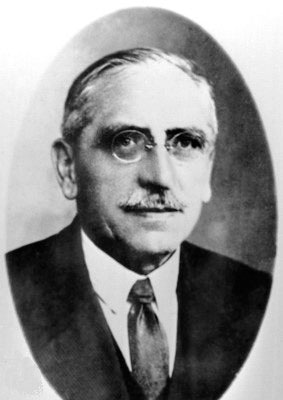
\includegraphics[width=3cm]{lebesgue.jpeg}
    \caption{Henri Lebesgue (1875 -- 1941)}
\end{figure}

Nesta seção, abordaremos os conceitos fundamentais da integral de Lebesgue, destacamos importância aos teoremas da convergência monotona e convergência dominada.
Vale ressaltar que nessa seção estaremos trabalhando em um espaço de medida $(X, \mathfrak{M}, \mu)$ fixo.

\begin{dbox}
    Uma função $\varphi : X \to \bR$ é simples se assume apenas um número finito de valores em sua imagem ($\# \varphi(X) < \infty$)
\end{dbox}

Uma função $\varphi$ simples e mensurável pode ser representada da seguinte forma
\begin{equation} \label{eq:representacaopadrao}
    \varphi = \sum_{j = 1}^n a_j \chi_{E_j}
\end{equation}
onde $a_j \in \bR$ e $\chi_{E_j}$ é a função caracteristica do conjunto $E_j \in \eth$. Essa representação é única pelo fato de todos $a_j$ serem distintos, os conjuntos $E_j$ serem disjuntos para todo $j = 1,\dots,n$, além disso, $X = \bigcup_{j=1}^n E_j$.    

\begin{dbox}
    Seja $\varphi \in \cM^+(X,\eth)$ uma função simples com a representação (\ref{eq:representacaopadrao}). Definimos a integral de $\varphi$ em relação a $\mu$ por
    \begin{equation*}
        \int \varphi \, d\mu = \sum_{j=1}^n a_j \mu(E_j)
    \end{equation*}
\end{dbox}

\obs Adotamos a convenção $0 \cdot \infty = 0$. Dessa forma a integral da função identicamente nula é $0$ indepdendente se o conjunto tem medida finita ou infinita.

\begin{lbox} \label{lm:propiedades-elementares-simples}
    Dadas funções simples $\varphi, \psi \in M^+(X, \eth)$ e $c \geqslant 0$ tem-se
    \begin{enumerate}[leftmargin=*, label=\textbf{(\alph*)}]
        \item $\displaystyle \int c \varphi \, d\mu = c \int \varphi \, d\mu$
        \item $\displaystyle \int (\varphi + \psi) \, d\mu = \int \varphi \,d\mu + \int \psi \, d\mu$
        \item A aplicação
        $\displaystyle \lambda(E) = \int \varphi \chi_E \, d\mu$
        para todo $E \in \eth$ é uma medida em $\eth$.
    \end{enumerate}
\end{lbox}
\begin{prf}
    ~

    \textbf{(a)} Mostremos que
    \[
        \int c \varphi \, d\mu = c \int \varphi \, d\mu.
    \]
    Com efeito, para $c = 0$,
    \[
        \int c \varphi \, d\mu = 0 = c \int \varphi \, d\mu.
    \]
    por outro lado, para $c > 0$, podemos escrever $c\varphi$ da seguinte forma
    \[
        c\varphi = \sum_{j = 1}^{n} ca_j \chi_{E_j}
    \]
    Dito isso,
    \[
        \int c \varphi \, d\mu = \sum_{j = 1}^{n} ca_j \mu(E_j) = c\sum_{j = 1}^{n} a_j \mu(E_j) = c\int \varphi \, d\mu
    \]

    \textbf{(b)} Agora, mostremos que 
    \[
        \int (\varphi + \psi) \, d\mu = \int \varphi \,d\mu + \int \psi \, d\mu
    \]
    Para isso, podemos considerar as representações padrões das funções simples $\varphi, \psi \in \cM^+(X,\eth)$
    \[
        \varphi = \sum_{j = 1}^{n} a_j \chi_{E_j} \quad \text{ e } \quad \psi = \sum_{k = 1}^{m} b_k \chi_{F_k},
    \]
    dessa forma, obtemos uma representaçao para $\varphi + \psi$ dada por
    \[
        \varphi + \psi = \sum_{j = 1}^{n} a_j \chi_{E_j} + \sum_{k = 1}^{m} b_k \chi_{F_k}.
    \]
    No entanto, essa representação não necessáriamente é a representação padrão, pois é possível que existam $j_0, j_1 \in \{1,\dots,n\}$ e $k_0, k_1 \in \{1,\dots,m\}$, tais que $a_{j_0} + b_{k_0} = a_{j_1} + b_{k_1}$.

    Considere os elementos distintos do conjunto
    \[
        H = \{a_j + b_k \,; j \in \{1,\dots,n\}, k \in \{1,\dots,m\}\}
    \]
    e denominamos os elementos por $c_h$ com $h = 1,\dots,\# H$, e $G_h$ a união de todos os conjuntos $E_j \cap F_k$ tais que $a_j + b_k = c_h$

    Afirmamos que os conjuntos $G_h$ são dois-a-dois disjuntos. De fato
    \[
        G_h \cap G_H = (E_j \cap F_k) \cap (E_J \cap F_K) = E_j \cap E_J \cap F_k \cap F_K = \emptyset \cap \emptyset = \emptyset,
    \]
    sendo assim
    \[
        \mu(G_h) = \widetilde{\sum} \mu(E_j \cap F_k)
    \]
    onde o somatório $\widetilde{\Sigma}$ está relacionado aos indices $1 \leqslant j \leqslant n$ e $1 \leqslant k \leqslant m$ tais que $a_j + b_k = c_h$

    Portanto definimos a representação padrão de $\varphi + \psi$ por
    \[
        \varphi + \psi = \sum_{h = 1}^{\# H} c_h \chi_{G_h},
    \]
    deste modo
    \[
        \begin{aligned}
            \int (\varphi + \psi) \, d\mu &= \sum_{h = 1}^{\# H} c_h \textcolor{ForestGreen}{\mu(G_h)}\\
            &= \sum_{h = 1}^{\# H} \textcolor{ForestGreen}{\widetilde{\sum}} c_h \textcolor{ForestGreen}{\mu (E_j \cap F_k)}\\
            &= \sum_{j = 1}^{n} \sum_{k = 1}^{m} (a_j + b_k) \mu(E_j \cap F_k)\\
            &= \sum_{j = 1}^{n} \sum_{k = 1}^{m} a_j \mu(E_j \cap F_k) + \sum_{j = 1}^{n} \sum_{k = 1}^{m} b_k \mu(E_j \cap F_k)
        \end{aligned}
    \]
    como $X$ é a união das famílias $\{E_j\}$ e $\{F_k\}$, temos que
    \[
        \mu(E_j) = \sum_{k = 1}^{m} \mu(E_j \cap F_k) \quad{ e } \quad \mu(F_k) = \sum_{j = 1}^{n} \mu(E_j \cap F_k).
    \]
    Portanto
    \[
        \int (\varphi + \psi) \, d\mu = \sum_{j = 1}^{n}  a_j \mu(E_j) + \sum_{k = 1}^{m}  b_k \mu(F_k) = \int \varphi \, d\mu + \int \psi \, d\mu.
    \]

    \textbf{(c)} Por fim, queremos mostrar que
    \[
        \lambda(E) = \int \varphi \chi_E \, d\mu
    \]
    é uma medida em $\eth$. Com efeito,
    \begin{enumerate}
        \item $\displaystyle \lambda (\emptyset) = \int \varphi \chi_{\emptyset} \, d\mu = \int 0 \, d\mu = 0$
        \item Note que como $\varphi \in \cM^+(X,\eth)$ os elementos $a_j$ na representação padrão são não negativos. Com efeito, sabemos que $0 \leqslant \varphi(x)$ para todo $x \in X$, daí
        \[
            0 \leqslant \varphi(x) = \sum_{j=1}^{n} a_j \chi_{E_j}(x),
        \]
        porem, como os conjuntos $E_j$ são disjuntos, existe um único $1 \leqslant j_0 \leqslant n$ tal que $x \in E_{j_0}$. 
        Dessa forma, para todo $j \neq j_0$, $\chi_{E_j}(x) = 0$, então
        \[
            0 \leqslant \varphi(x) = \sum_{j=1}^{n} a_j \chi_{E_j}(x) = a_{j_0}
        \]
        Daí,
        \[
            \lambda(E) = \int \varphi \chi_{E} \, d\mu = \sum_{j=1}^{n} a_j \mu(E \cap E_j) \geqslant 0
        \]
        pois mostramos que $a_j > 0$ para todo $1 \leqslant j \leqslant n$ e $\mu$ é uma medida.
        \item Considere $(F_k) \subseteq \eth $ uma sequência disjunta de conjuntos
        \[
            \begin{aligned}
                \lambda \left( \bigcup_{k=1}^\infty F_k \right) &= \int \varphi \chi_{\medcup F_k}\\ 
                &= \sum_{j = 1}^{n} a_j \mu \left( \left( \bigcup_{k = 1}^\infty F_k \right) \cap E_j \right)\\
                &= \sum_{j = 1}^{n} a_j \mu \left( \bigcup_{k=1}^\infty (F_k \cap E_j) \right)\\
                &= \sum_{j=1}^{n} a_j \sum_{k=1}^{\infty} \mu(F_k \cap E_j)\\
                &= \sum_{j=1}^{n}\sum_{k=1}^{\infty} a_j  \mu(F_k \cap E_j)\\
                &= \sum_{k=1}^{\infty}\sum_{j=1}^{n} a_j  \mu(F_k \cap E_j)\\
                &= \sum_{k=1}^{\infty} \int \varphi \chi_{F_k} \, d\mu\\
                &= \sum_{k=1}^{\infty} \lambda(F_k)
            \end{aligned}
        \]
    \end{enumerate}
\end{prf}

Agora, podemos extender a definição da integral de Lebesgue para qualquer função mensurável não negatíva (não necessáriamente simples)

\begin{dbox}
    A integral de uma função $f \in \cM^+(X,\eth)$ em relação a $\mu$ é definida por
    \[
        \int f \, d\mu = \sup_\varphi \int \varphi \, d\mu
    \]
    onde $\varphi$ são funções simples em $\mathcal{M}^+(X,\eth)$ tais que $0 \leqslant \varphi(x) \leqslant f(x)$ para todo $x \in X$.
\end{dbox}

Além disso, definimos a integral da função $f$ sobre um conjunto mensurável

\begin{dbox}
    A integral de $f \in \cM^+(X,\eth)$ sobre um conjunto $E \in \eth$ é dada por
    \[
        \int_E f \, d\mu = \int f \chi_E \, d\mu
    \]
\end{dbox}

\dots

\begin{lbox} \label{lm:propiedades-integral-nao-negativa}
    Sejam $f, g \in \cM^+(X,\eth)$ e $E, F \in \eth$.
    Então são válidas as afirmações abaixo
    \begin{enumerate}[leftmargin=*, label=\textbf{(\alph*)}]
        \item se $f \leqslant g$ tem-se
        \[
            \int f \, d\mu \leqslant \int g \, d\mu
        \]
        \item se $E \subseteq F$ tem-se
        \[
            \int_E f \, d\mu \leqslant \int_F f \, d\mu
        \]
    \end{enumerate}
\end{lbox}
\begin{prf}
    ~

    \textbf{(a)} Seja $\varphi$ uma função simples em $M^+$, então
    \[
        \int f \, d\mu = \sup_{\substack{0 \leqslant \varphi \leqslant f \\ \varphi \text{ simples} \\ \varphi \in M^+}} \int \varphi \, d \mu \leqslant \sup_{\substack{0 \leqslant \varphi \leqslant g \\ \varphi \text{ simples} \\ \varphi \in M^+}} \int \varphi \, d \mu = \int g \, d\mu
    \]

    \textbf{(b)} Como $f \chi_E \leqslant f \chi_F$, segue do item anterior que
    \[
        \int f \chi_E \, d\mu \leqslant \int f \chi_F \, d\mu,
    \]
    dito isso
    \[
        \int_E F \, d \mu \leqslant \int_F f \, d\mu.
    \]
\end{prf}

Um dos resultados mais importantes da teoria da medida é o Teorema da Convergência Monótona, que será enunciado e demonstraado a seguir.

\begin{tbox}[Teorema da Convergência Monótona] \label{thm:teorema-da-convergencia-monotona}
    Seja $(f_n)$ uma sequência monótona crescente de funções mensuráveis não-negativas convergindo para $f$, então,
    \[
        \int f \, d\mu = \lim \int f_n \, d \mu.
    \]
\end{tbox}
\begin{prf}
    Como $f_n \to f$ onde $(f_n) \subseteq \cM^+(X,\eth)$, pelo corolário ?? temos que $f \in \cM^+(X,\eth)$.
    Pela monotonicidade da sequência $f_n \leqslant f_{n+1} \leqslant f$, pelo item \textbf{(a)} do lema anterior
    \[
        \int f_n \, d\mu \leqslant \int f_{n+1} \, d\mu \leqslant \int f \, d\mu
    \]
    para todo $n \in \bN$. 
    Dito isso
    \[
        \lim \int f_n \, d\mu \leqslant \int f \, d\mu.
    \]

    Por outro lado, seja $0 < \alpha < 1$ e $\varphi$ uma função simples mensurável tal que $0 \leqslant \varphi \leqslant f$ e considere
    \[
        A_n = \{x \in X \,; f_n(x) \geqslant \alpha \varphi(x)\} = \{x \in X \,; [f_n - \alpha \varphi](x) \geqslant 0\}
    \]
    como $f_n$ e $\varphi$ são funções mensuráveis, temos que $A_n \in \eth$.
    Além disso, $A_n \subseteq A_{n+1}$ já que $f_n \leqslant f_{n+1}$ e $X = \bigcup_{n =1}^{\infty} A_n$ pois $\sup \{f_n\} = f$, $\alpha \in (0,1)$ e $0 \leqslant \varphi \leqslant f$.
    Daí, pelo lema anterior
    \begin{equation} \label{eq:1.13}
        \int_{A_n} \alpha \varphi \,d\mu \leqslant \int_{A_n} f_n \, d\mu \leqslant \int f_n \, d\mu.
    \end{equation}
    Dessa forma, a sequência $(A_n)$ é monótona crescente e tem união $X$, segue dos lemas ?? e ?? que
    \[
        \int \varphi \, d\mu = \lim \int_{A_n} \varphi \, d\mu
    \]
    Com efeito, sabemos que
    \[
        \lambda(E) = \int \varphi \chi_{E} \, d \mu
    \]
    é uma medida, assim
    \[
        \int \varphi \, d\mu = \int \varphi \chi_{\medcup A_n} \, d\mu = \lambda \left( \bigcup_{n=1}^\infty A_n \right) = \lim \lambda(A_n) = \lim \int \varphi \chi_{A_n} \, d\mu = \lim \int_{A_n} \varphi \, d\mu
    \]
    ... fazendo $n \to \infty$ em \ref{eq:1.13}
    \[
        \alpha \int \varphi \, d\mu \leqslant \lim \int f_n \, d\mu.
    \]
    Como a equação acima é válida para todo $0 < \alpha < 1$, obtemos
    \[
        \int \varphi \, d\mu \leqslant \lim \int f_n \, d\mu,
    \]
    ainda mais, segue do fato de $\varphi$ ser uma função simples tal que $0 \leqslant \varphi \leqslant f$ tem-se que
    \[
        \int f \, d\mu = \sup_{\substack{0 \leqslant \varphi \leqslant f \\ \varphi \text{ simples} \\ \varphi \in M^+}} \int \varphi \, d\mu \leqslant \lim \int f_n d \mu.
    \]
    Assim
    \[
        \int f \, d\mu \leqslant \lim \int f_n \, d\mu
    \]
    Portanto por ?? e ??, chegamos a
    \[
        \int f \, d\mu = \lim \int f_n \, d\mu
    \]
\end{prf}

O Lema \ref{lm:propiedades-elementares-simples} sobre as operações elementares envolvendo a integral de funções simples mensuráveis e não-negativas, tambem é válido para funções mensuráveis não-negativas quaisquer como mostra o corolário abaixo

\begin{cbox} \label{cl:propiedades-elementares-nao-negativa}
    Sejam $f, g \in \cM^+(X,\eth)$ e $c > 0$, então são válidas as seguintes afirmações
    \begin{enumerate}[leftmargin=*, label=\textbf{(\alph*)}]
        \item $\displaystyle \int cf \, d\mu = c \int f \,d \mu$
        \item $\displaystyle \int (f + g) \, d\mu = \int f \,d \mu + \int g \, d\mu$
    \end{enumerate}
\end{cbox}
\begin{prf}
    ~

    \textbf{(a)} Se $c = 0$
    \[
        \int c f \, d\mu = 0 = c \int f \, d\mu.
    \]
    Se $c > 0$, considere $(\varphi_n)$ uma sequência monótona crescente de funções simples em $\cM^+(X,\eth)$ convergindo para $f$ (lema ??). Dito isso, $(c\varphi_n)$ é um sequência monótona crescente que converge para $cf$. Pelo Lema \ref{lm:propiedades-elementares-simples} e pelo Teorema da Convergência Monótona, temos que
    \[
        \int cf \, d\mu = \lim \int c \varphi_n \, d\mu = c \lim \int \varphi_n \, d\mu = c \int f \, d\mu.
    \]

    \textbf{(b)} De forma análoga considere $(\varphi_n)$ e $(\psi_n)$ sequências monótonas crescentes de funçoes simplies em $\cM^+(X,\eth)$ que convergem para $f$ e $g$ respectivamente. Dessa forma $(\varphi_n + \psi_n)$ é uma sequência monótona crescente que converge para $f + g$. Portanto
    \[
        \int (f+g) \, d\mu = \lim \int (\varphi_n + \psi_n) \, d \mu = \lim \int \varphi_n \, d\mu + \lim\int \psi_n \, d\mu = \int f \, d\mu + \int g \, d\mu.
    \]
\end{prf}

Um outro resultado importante dessa seção é o lema de Fatou que será apresentado a seguir.

\begin{lbox}[Lema de Fatou] \label{lm:lema-de-fatou}
    Se $(f_n) \subseteq M^+ (X,\eth)$, então
    \[
        \int\liminf f_n \, d\mu\leqslant\liminf \int f_n \,d\mu.
    \]
\end{lbox}
\begin{prf}
    Seja $g_m = \inf \{ f_m, f_{m+1},\dots\}$, dessa forma $g_m \leqslant f_n$ para todo $m \leqslant n$.
    Sendo assim,
    \[
        \int g_m \, d\mu \leqslant \int f_n \, d\mu
    \]
    para todo $m \leqslant n$. Desse modo
    \[
        \int g_m \,d\mu \leqslant \liminf \int f_n \, d\mu.
    \]
    Por outro lado, temos que $(g_m)$ é crescente e converge para seu supremo, ou seja, $\liminf f_n$.
    Portanto pelo \nameref{thm:teorema-da-convergencia-monotona}
    \[
        \int \liminf f_n \, d\mu = \lim \int g_m \,d\mu \leqslant \liminf \int f_n\, d\mu.
    \]
\end{prf}

Da mesma forma que definimos uma medida através de uma função simples em $\cM^+(X,\eth)$ podemos generalizar esse resultado para funções que não são necessáriamente simples

\begin{cbox} \label{cl:medida-funcao-nao-negativa}
    Seja $f \in \cM^+(X,\eth)$.
    A aplicação $\lambda : \eth \to \overline\bR$ definida por
    \[
        \lambda(E) = \int f \chi_E \, d\mu 
    \]
    é uma medida.
\end{cbox}
\begin{prf}
    ~

    \begin{enumerate}
        \item $\displaystyle\lambda(\emptyset) = \int_{\emptyset} f \, d\mu = \int f \chi_{\emptyset} \, d\mu = \int 0  \, d\mu = 0$.
        
        \item Como $f \in \cM^+(X,\eth)$ temos que $\lambda(E) = \int_E f \, d\mu \geqslant \int_E 0 \, d\mu = 0$.

        \item Sejam $E_n$ uma sequência de conjuntos disjuntos em $\eth$, $E = \bigcup_{n=1}^{\infty} E_n$ e considere $f_n$ definida por
        \[
            f_n = \sum_{k=1}^{n} f \chi_{E_k}
        \]
        Desse modo, pelo Corolário ?? e por indução temos que
        \[
            \int f_n \, d\mu = \int \sum_{k=1}^{n} f \chi_{E_k} \, d\mu = \sum_{k=1}^{n} \int f \chi_{E_k} = \sum_{k=1}^{n} \lambda(E_k).
        \]
        Além diso, podemos escrever
        \[
            \lim f_n = \lim \sum_{k=1}^{n} f \chi_{E_k} = \sum_{k=1}^{\infty} f \chi_{E_k} = f \chi_E
        \]
        desde que $(E_n)$ é uma sequência de conjuntos disjuntos.

        Por fim, como $(f_n)$ é uma sequência crescente em $M^+$ que converge para $f \chi_E$, pelo Teorema da Convergência Monótona tem-se que
        \[
            \lambda(E) = \int f \chi_E \, d\mu = \int \lim f_n \,d\mu = \lim \int f_n \, d\mu = \sum_{k=1}^{\infty} f \chi_{E_k}
        \]
    \end{enumerate}
    Portanto, $\lambda$ é uma medida.
\end{prf}

\begin{cbox} \label{cl:integral-medida-nula}
    Seja $f \in \cM^+(X,\eth)$.
    Então, $f(x) = 0$ em quase toda parte de $X$ se, e somente se,
    \[
        \int f \, d\mu = 0
    \]
\end{cbox}
\begin{prf}
    Suponha que $\displaystyle \int f\,d\mu = 0$ e considere o conjunto
    \[
        E_n = \left\{ x \in X \,; f(x) > \frac{1}{n} \right\}
    \]
    para todo $n \in \bN$, de modo que $f \geqslant \frac{1}{n}\chi_{E_n}$.
    Note que
    \[
        0 = \int f \,d\mu \geqslant \tfrac{1}{n} \! \int \chi_{E_n} \, d\mu = \tfrac{1}{n}\mu(E_n) \geqslant 0.
    \]
    Isto nos diz que $\mu(E_n) = 0$ para todo $n \in \bN$. Além disso
    \[
        E = \{x \in X \,; f(x) > 0\} = \bigcup_{n=1}^{\infty} E_n
    \]
    pois se $x \in \bigcup_{n=1}^{\infty} E_n$, então existe $n_0 \in \bN$ tal que $x \in E_{n_0}$, logo
    \[
        f(x) > \frac{1}{n_0} > 0.
    \]
    Assim, $x \in E$.\\[5pt]
    Por outro lado, se $x \in E$, temos que $f(x) > 0$.
    Utilizando a propiedade Arquimediana, existe $n_0 \in \bN$ tal que
    \[
        \frac{1}{f(x)} < n_0 \iff f(x) > \frac{1}{n_0},
    \]
    isto é, $x \in E_{n_0} \subseteq \bigcup_{n=1}^{\infty} E_n$.\\[5pt]
    Portanto $E = \bigcup_{n=1}^{\infty} E_n$ como queriamos mostrar. Dito isso
    \[
        \mu(E) = \mu\left( \bigcup_{n=1}^{\infty} E_n \right) = \lim \mu(E_n) = 0
    \]
    desde que $(E_n)$ é uma sequência crescente.
    Isto nos diz que $f(x) = 0$, para todo $x \in E^{\cC}$ com $\mu(E) = 0$, ou seja $f(x) = 0$ em quase toda parte em $X$.

    Reciprocamente, suponha que $f(x) = 0$ em quase toda parte em $X$. Se $E = \{x \in X \,; f(x) > 0\}$, então $\mu(E) = 0$.
    Sendo assim, considerando $f_n = n \chi_E$ para todo $n \in \bN$, temo que $f \leqslant \liminf f_n$ e pelo Lema de Fatou
    \[
        0 \leqslant \int f \, d\mu \leqslant \liminf \int f_n \,d\mu = \liminf n\mu(E) = 0
    \]
    Portanto
    \[
        \int f \, d\mu = 0.
    \]
\end{prf}

\begin{cbox} \label{cl:medida-absolutamente-continua}
    Seja $f \in \cM^+(X,\eth)$, então a aplicação $\lambda : \eth \to \bR$ definida por
    \[
        \lambda(E) = \int_E f \, d\mu.
    \]
    Então, a medida $\lambda$ é absolutamente contínua em relação a $\mu$, isto é, se $\mu(E) = 0$, então $\lambda(E) = 0$
\end{cbox}
\begin{prf}
    Se $\mu(E) = 0$, então
    \[
        f\chi_E(x) = 
        \left\{
            \begin{array}{cl}
                f(x) & x \in E\\
                0 & x \not\in E
            \end{array}
        \right.
    \]
    isto é, $f \chi_E = 0$ em quase toda parte. Portanto
    \[
        \lambda(E) = \int_E f \,d\mu = \int f\chi_E \, d\mu = 0.
    \]
\end{prf}

O corolário abaixo é uma versão mais geral do Teorema da Convergência Monótona.

\begin{cbox} \label{cl:convergencia-monotona-qtp}
    Se $(f_n)$ é uma sequência monótona crescente de funções em $\cM^+(X,\eth)$ que converge em quae toda parte de $X$ para a função $f \in \cM^+(X,\eth)$, então
    \[
        \int f \, d\mu = \lim \int f_n \, d\mu
    \]
\end{cbox}
\begin{prf}
    Seja $N$ um conjunto de medida nula. Suponha que $(f_n)$ converge para $f$ em todo o pontos de $M = N^{\cC}$.
    Dessa forma, a sequência $(f_n \chi_M)$ converge para $f\chi_M$, pelo Teorema da Convergência Monótona, temos que
    \[
        \int f \chi_M \, d\mu = \lim \int f_n \chi_M \, d\mu.
    \]
    Além disso, podemos escrever $f$ e $f_n$ da seguinte forma
    \[
        f = f \chi_M + f \chi_N \;\text{ e }\; f_n = f_n \chi_M + f_n \chi_N,
    \]
    pois $M = N^{\cC}$.
    Como $\mu(N) = 0$, as funções $f \chi_N$ e $f_n \chi_N$ são nulas em quase toda parte.
    Dito isso, pelo Corolário \ref{cl:integral-medida-nula}, segue que
    \[
        \lim \int f_n \, d\mu = 
    \]
\end{prf}

O resultado abaixo ...

\begin{cbox}
    Seja $(g_n)$ uma sequência em $\cM^+(X,\eth)$. Então
    \[
        \int \left( \sum_{n=1}^{\infty} g_n \right) \, d\mu = \sum_{n=1}^{\infty} \int g_n \, d\mu.
    \]
\end{cbox}
\begin{prf}
    Seja $f_n = g_1 + \cdots + g_n$ para todo $n \in \bN$. Como $g_n \geqslant 0$, temos que $(f_n)$ é uma sequência crecente que converge para $f = \sum_{n=1}^{\infty} g_n$. 
    Pelo Teorema da Convergência Monótona, segue que
    \[
        \lim_{k \to \infty} \int \left( \sum_{n=1}^{k} g_n \right) \, d\mu = \lim_{k\to\infty} \int f_k \, d \mu = \int f \, d\mu = \int \left( \sum_{n=1}^{\infty} g_n \right) \, d\mu.
    \]
    Por outro lado, como $g_n \in \cM^+(X,\eth)$, para todo $n \in \bN$, utilizando indução e o Corolário ??
    \[
        \lim_{k \to \infty} \int \left( \sum_{n=1}^{k} g_n \right) \,d\mu = \lim_{k\to \infty} \sum_{n=1}^{k} \int g_n \, d\mu = \sum_{n=1}^{\infty} \int g_n \, d\mu
    \]
    Portanto
    \[
        \int \left( \sum_{n=1}^{\infty} g_n \right) \, d\mu = \sum_{n=1}^{\infty} \int g_n \, d\mu.
    \]
\end{prf}

Finalmente, podemos definir a integral de uma função mensurável qualquer

\begin{dbox}
    O conjunto $\cL(X,\eth,\mu)$ das funções integráveis consite em todas as funções $f : X \to \bR$ mensuráveis, tai que as integrais
    \[
        \int f^+ \,d\mu \;\text{ e }\; \int f^- \,d\mu
    \]
    são finitas.
    Neste caso, definimos a integral de $f$ em relação a $\mu$ por
    \[
        \int f \, d\mu = \int f^+ \, d\mu - \int f^- \, d\mu,
    \]
    e se $E$ é um conjunto mensurável
    \[
        \int_E f \, d\mu = \int_E f^+ \, d\mu - \int_E f^- \, d\mu.
    \]
\end{dbox}

Qualquer representação de $f$ como subtrações de funções integráveis não-negativas resulta no mesmo valor da integral da definição acima.
Com efeito seja $f$ uma função integravel e escreva $f$ como $f = f_1 - f_2$, onde $f_1$ e $f_2$ são funções integráveis não negativas, então
\[
    \int f \,d\mu = \int f_1 \, d\mu - \int f_2 \,d \mu.
\]
Note que
\[
    f^+ - f^- = f = f_1 - f_2 \iff f^+ + f_2 = f_1 + f^-.
\]
Dessa forma, pelo Corolário ?? temos que
\[
    \int f^+ \,d\mu + \int f_2 \, d\mu = \int f_1\,d\mu + \int f^- \, d\mu.
\]
Como $f_1, f_2, f^+,f^- \in \cL(X,\eth,\mu)$, segue que
\[
    \int f^+ \,d\mu - \int f^- \, d\mu = \int f_1 \,d\mu - \int f_2 d\mu.
\]
Isto é
\[
    \int f \, d\mu = \int f_1 \,d\mu + \int f_2 \,d\mu.
\]

Da mesma forma que definimos um medida a partir da integral de uma função não-negativa, podemos definir uma carga partindo da integral de uma função integrável qualquer como exibe o lema abaixo

\begin{lbox} \label{lm:carga-integral}
    Seja $f \in \cL(X,\eth,\mu)$. A aplicação $\lambda : \eth \to \bR$ definida por
    \[
        \lambda(E) = \int_E f \, d\mu
    \]
    é uma carga, denominada integral indefinida de $f$ (em relação a $\mu$).
\end{lbox}
\begin{prf}
    Como $f^+, f^- \in M^+(X,\eth,\mu)$, pelo Corolário ?? temos que as funções $\lambda^+, \lambda^- : \eth \to \bR$ dadas por
    \[
        \lambda^+(E) = \int_E f^+ \,d\mu \;\text{ e }\; \lambda^-(E) = \int_E f^- \,d\mu.
    \]
    são medidas em $\eth$ e são finitas pelo fato de $f$ ser uma função integrável. Como $\lambda = \lambda^+ - \lambda^-$ temos que $\lambda$ é uma carga.
\end{prf}

Como a aplicação $\lambda$ definida acima é uma carga, vemos que se $(E_n)$ é uma sequência de conjuntos disjuntos tal que $\bigcup_{n=1}^{\infty} E_n = E$, então
\[
    \int_E f \,d\mu = \lambda(E) = \lambda \left( \bigcup_{n=1}^{\infty} E_n \right) = \sum_{n=1}^{\infty} \lambda(E_n) = \sum_{n=1}^{\infty} \int_{E_n} f\,d\mu,
\]
ou seja
\[
    \int_E f \, d\mu = \sum_{n=1}^{\infty} \int_{E_n} f\,d\mu
\]

Agora, estamos prontos para estudar algumas propiedades elementares das integrais de funções mensuráveis

\begin{tbox} \label{thm:modulo-funcao-integravel}
    Seja $f : X \to \bR$ uma função mensurável.
    Então $f \in \cL(X,\eth,\mu)$ se, e somente se, $|f| \in \cL(X,\eth,\mu)$.
    Além disso
    \begin{equation} \label{eq:desigualdade-modulo-integral}
        \left\vert \int f \,d\mu \right\vert \leqslant \int |f| \,d\mu.
    \end{equation}
\end{tbox}
\begin{prf}
    Seja $f$ uma função integrável, mostremos que $|f|$ também o é.
    Primeiramente note que
    \[
        |f|^+ = |f| = f^+ + f^- \;\text{ e }\; |f|^- = 0,
    \]
    Dito isso
    \[
        \int |f|^+ \,d\mu = \int f^+ \,d\mu + \int f^- \,d\mu
    \]
    é finita pois $f$ é integrável, e
    \[
        \int |f|^- \,d\mu = \int 0 \,d\mu = 0
    \]
    que é finita.
    Portanto $|f|$ é integrável.

    Reciprocamente, suponha que $|f|$ é integrável, dessa forma
    \[
        \begin{aligned}
            f^+ &\leqslant f^+ + f^- = |f|\\
            f^- &\leqslant f^+ + f^- = |f|
        \end{aligned}
    \]
    sendo assim
    \[
        \begin{aligned}
            \int f^+ \,d\mu &\leqslant \int |f| \,d\mu\\
            \int f^- \,d\mu &\leqslant \int |f| \,d\mu
        \end{aligned}
    \]
    ambas finitas pois $|f|$ é integrável.
    Portanto $f$ é integrável.

    Para mostrar a desigualdade (\ref{eq:desigualdade-modulo-integral}) basta utilizar a definição de função integravel e a desigualdade triangular.
    \[
        \left\vert \int f \,d\mu \right\vert = \left\vert \int f^+ \,d\mu - \int f^- \,d\mu \right\vert \leqslant \left\vert \int f^+ \,d\mu \right\vert + \left\vert \int f^- \,d\mu \right\vert = \int f^+ \,d\mu + \int f^- \,d\mu = \int |f| \,d\mu
    \]
\end{prf}

\begin{cbox} \label{cl:g-implica-f-integravel}
    Se $f \in \cM(X,\eth)$, $g \in \cL(X,\eth,\mu)$ e $|f| \leqslant |g|$, então $f \in \cL(X,\eth,\mu)$ e 
    \[
        \int |f| \,d\mu \leqslant \int |g| \,d\mu
    \]
\end{cbox}
\begin{prf}
    Se $g$ é integrável então pelo Teorema anterior $|g|$ também o é.
    Além disso, como $|f| \leqslant |g|$
    \[
        \int |f| \,d\mu \leqslant \int |g| \,d\mu,
    \]
    como $|g|$ é integrável a sua integral é finita, implicando na integral de $|f|$ também ser finita, ou seja, $|f|$ é integrável e novamente pelo Teorema anterior, $f$ é integrável.
\end{prf}

\begin{tbox} \label{thm:operacoes-elementares-integral}
    Sejam $f, g \in \cL(X,\eth,\mu)$ e $c \in \bR$, então $cf, f + g \in \cL(X,\eth,\mu)$ e 
    \begin{enumerate}[leftmargin=*, label=\textbf{(\alph*)}]
        \item $\displaystyle \int cf \, d\mu = c \int f \,d \mu$
        \item $\displaystyle \int (f + g) \, d\mu = \int f \,d \mu + \int g \, d\mu$
    \end{enumerate}
\end{tbox}
\begin{prf}
    ~

    \textbf{(a)} Se $c \geqslant 0$.
    Note que $(cf)^+ = c f^+$ e $(cf)^- = cf^-$. Dito isso
    \[
        \int cf \,d\mu = \int cf^+ - cf^- \,d\mu 
    \]
    como $cf^+$ e $cf^-$ são funções mensuráveis não negativas, podemos utilizar o Corolário \ref{cl:propiedades-elementares-nao-negativa}
    \[
        \int cf \,d\mu =  c \int f^+ - f^- \,d\mu = c \int f\,d\mu
    \]

    Se $c < 0$ a demonstração é análoga, basta perceber que $(cf)^+ = -c f^-$ e $(cf)^- = -cf^+$ ambas funções não negativas pois $-c > 0$.

    \textbf{(b)} Sejam $f, g \in \cL(X,\eth,\mu)$, então pelo Teorema \ref{thm:modulo-funcao-integravel} $|f|, |g| \in \cL(X,\eth,\mu)$, como $| f + g| \leqslant |f| + |g|$ temos que $f + g$ é integrável. Note que
    \[
        f + g = f^+ - f^- + g^+ - g^- = (f^+ + g^+) - (f^- + g^-),
    \]
    onde $f^+ + g^+$ e $f^- + g^-$ são funções integráveis não negativas. Dessa forma
    \[
        \int (f + g)\,d\mu = \int (f^+ + g^+)\,d\mu - \int (f^- + g^-)\,d\mu
    \]
    Utilizando o Corolário \ref{cl:medida-funcao-nao-negativa} e reorganizando os termos
    \[
        \begin{aligned}
            \int (f + g)\,d\mu &= \int f^+ \,d\mu + \int g^+\,d\mu - \int f^- \,d\mu  -\int g^-\,d\mu\\
            &= \int f^+ \,d\mu  - \int f^- \,d\mu + \int g^+ \,d\mu  - \int g^- \,d\mu\\
            &= \int f \,d\mu + \int g \,d\mu.
        \end{aligned}
    \] 
\end{prf}

O teorema a seguir é um dos mais importantes da teoria da medida, envolvendo convergência de sequência de funções e integrais.

\begin{tbox}[Teorema da Convergência Dominada] \label{thm:teorema-da-convergencia-dominada}
    Seja $(f_n)$ uma sequência de funções integráveis que converge em quase toda parte para a função mensurável $f$.
    Se existe uma função integrável $g$ tal que $|f_n| \leqslant g$ em quase toda parte, para todo $n \in \bN$, então $f$ é integrável e
    \[
        \int f \,d\mu = \lim \int f_n \,d\mu.
    \]
\end{tbox}
\begin{prf}
    Redefinindo as funções $f_n$ e $f$ no conjunto de medida nula, podemos afirmar que a convergência acontece em todo $X$. Note que
    \[
        \lim |f_n| \leqslant g \implies |f| \leqslant |g|,
    \]
    como por hipótese $f$ é mensurável e $g$ é integrável, segue pelo Corolário \ref{cl:g-implica-f-integravel} que $f$ é integrável.
    Além disso, como $-g \leqslant f_n \leqslant g$ temos que $g + f_n \geqslant 0$ para todo $n \in \bN$.
    Utilizando o \nameref{lm:lema-de-fatou} e o Teorema \ref{thm:modulo-funcao-integravel} temos que
    \[
        \begin{aligned}
            \int g \,d\mu + \int f \, d\mu &= \int (g + f) \,d\mu\\
            &= \int (g + \lim f_n) \,d\mu\\
            &= \int \lim (g + f_n) \,d\mu\\
            &= \int \liminf (g + f_n) \,d\mu\\
            &\leqslant \liminf \int (g + f_n) \,d\mu\\
            &= \liminf \left( \int g \, d\mu + \int f_n \,d\mu \right)\\
            &= \int g \,d\mu + \liminf \int f_n \,d\mu,
        \end{aligned}
    \]
    que implica em
    \begin{equation} \label{eq:liminf}
        \int f \,d\mu \leqslant \liminf \int f_n \,d\mu.
    \end{equation}

    Por outro lado, $g - f_n \geqslant 0$, de forma análoga mostramos que
    \begin{equation} \label{eq:limsup}
        \limsup \int f_n \,d\mu \leqslant \int f\,d\mu.
    \end{equation}
    Pelas desigualdades (\ref{eq:liminf}) e (\ref{eq:limsup})
    \[
        \limsup \int f_n \,d\mu \leqslant \int f \,d\mu \leqslant \liminf \int f_n \,d\mu,
    \]
    isto é\footnotemark
    \[
        \int f \,d\mu = \lim \int f_n \,d\mu.
    \]
    Finalizando a demonstração do teorema.
\end{prf}

\footnotetext{$\limsup x_n \leqslant x \leqslant\liminf x_n$ para todo $n \in \bN$ $\implies$ $\lim x_n = x$}

No restante da seção focaremos nossa atenção em funções $f : X \times [a,b] \to \bR$ onde a aplicação $x \mapsto f(x,t)$ é mensurável para todo $t \in [a,b]$.

\begin{cbox}
    Suponha que para algum $t_0 \in [a,b]$, tenhamos
    \[
        f(x,t_0) = \lim_{t\to t_0} f(x,t),
    \]
    para cada $x \in X$ e que existe uma função integrável $g : X\to\bR$ tal que $|f(x,t)| \leqslant g(x)$, para todo $x \in X$ e $t \in [a,b]$.
    Então
    \[
        \int f(x,t_0) \, d\mu(x) = \lim_{t \to t_0} \int f(x,t) \, d\mu(x)
    \]
\end{cbox}
\begin{prf}
    Seja $t_n$ uma sequência em $[a,b]$ que converge para $t_0$ e considere a sequência $(f_n)$ dada por $f_n(x) = f(x,t_n)$. 
    Então como $|f_n(x)| = |f(x,t_n)| \leqslant g(x)$ para todo $n \in \bN$ e $x \in X$ com $g$ integrável, segue pelo \nameref{thm:teorema-da-convergencia-dominada} que
    \[
        \begin{aligned}
            \int f(x,t_0) \,d\mu(x) &= \int \lim_{t\to t_0} f(x,t) \, d\mu(x)\\
            &= \int \lim f_n(x) \,d\mu(x)\\
            &= \lim \int f_n(x) \,d\mu(x)\\
            &= \lim \int f(x,t_n) \, d\mu(x)\\
        \end{aligned}
    \]
    Consequentemente,
    \[
        \int f(x,t_0) \, d\mu(x) = \lim_{t \to t_0} \int f(x,t) \, d\mu(x)
    \]
\end{prf}

Uma consequência imediata do corolário será apresentada abaixo

\begin{cbox}
    Se a aplicação $t \mapsto f(x,t)$ for contínua em $[a,b]$ para cada $x \in X$, e se existir uma função integrável $g : X \to \bR$ tal que $|f(x,t)| \leqslant g(x)$ para todo $x \in X$ e $t \in [a,b]$.
    Então a função $F$ dada por
    \[
        F(t) = \int f(x,t) \,d\mu(x)
    \]
    é contínua.
\end{cbox}
\begin{prf}
    Mostremos que $\lim_{t \to t_0} F(t) = F(t_0)$.
    Com efeito
    \[
        \lim_{t \to t_0} F(t) = \lim_{t\to t_0} \int f(x,t) \,d\mu(x) = \int f(x,t_0) \,d\mu(x) = F(t_0)
    \]
\end{prf}

\begin{cbox}
    Suponha que ara algum $t_0 \in [a,b]$, a função $x \to f(x,t_0)$ seja integrável em $X$, que $\partial_t f$ existe em $X \times [a,b]$ e que existe uma função integrável $g$ em $X$ tal que
    \[ 
        \left\vert \dfrac{\partial f}{\partial t}(x,t) \right\vert < g(x)
    \]
    para todo $x \in X$ e $t \in [a,b]$.
    Então a função $F$ definida por
    \[
        F(t) = \int f(x,t) \, d\mu(x)
    \]
    é diferenciável em $[a,b]$ e 
    \[
        \frac{\mathrm{d} F}{\mathrm{d}t}(t) = \int \dfrac{\partial f}{\partial t}(x,t) \,d\mu(x)
    \]
\end{cbox}
\begin{prf}
    Seja $(t_n)$ uma sequência em $[a,b]$ que converge para $t$, com $t \neq t_n$ para todo $n \in \bN$.
    Então, podemos escrever
    \[
        \dfrac{\partial f}{\partial t}(x,t) = \lim \frac{f(x,t_n) = f(x,t)}{t_n - t}
    \]
    para todo $x \in X$.
    Desde modo a função $x \mapsto \partial f/\partial t \,(x,t)$ é mensurável pois é o limite de funções mensuráveis.

    Agora seja $x \in X$.
    Pelo Teorema do Valor Médio, existe $s_0$, entre $t_0$ e $t$ tal que
    \[
        f(x,t) - f(x,t_0) = (t - t_0)\dfrac{\partial f}{\partial t} (x,s_0)
    \]
    Dessa forma, temos que
    \[
        |f(x,t)| = \left\vert f(x,t_0) + (t - t_0)\dfrac{\partial f}{\partial t}(x,s_0) \right\vert \leqslant |f(x,t_0)| + |t-t_0|\left\vert \dfrac{\partial f}{\partial t} (x,s_0) \right\vert
    \]
    Como $f$ é mensurável e a aplicação $x \mapsto |f(x,t_0)| + |t-t_0|\left\vert \partial f / \partial t \, (x,s_0) \right\vert$ é integrável, pois é a soma de funções integráveis. Pelo Corolário \ref{cl:g-implica-f-integravel} temos que $f$ é integrável.
    Por outro lado
    \[
        \frac{F(t_n) - F(t)}{t_n - t} = \int \frac{f(x,t_n) - f(x,t)}{t_n - t} \,d\mu(x)
    \]
    Além disso, por hipótese, podemos deduzir que
    \[
        \lim \left\vert \frac{f(x,t_n) - f(x,t)}{t_n - t} \right\vert =  \left\vert \lim\frac{f(x,t_n) - f(x,t)}{t_n - t} \right\vert = \left\vert \dfrac{\partial f}{\partial t}(x,t) \right\vert < g(x)
    \]
    para todo $x \in X$.
    Consequentemente
    \[
        \left\vert \frac{f(x,t_n) - f(x,t)}{t_n - t} \right\vert < g(x)
    \]
    para valores de $n$ suficientemente grande.
    Pelo \nameref{thm:teorema-da-convergencia-dominada}, temos
    \[
        \frac{\mathrm{d} F}{\mathrm{d}t}(t) = \lim \frac{F(t_n) - F(t)}{t_n - t} = \lim  \int \frac{f(x,t_n) - f(x,t)}{t_n - t} \,d\mu(x) = \int \dfrac{\partial f}{\partial t} (x,t) \, d\mu(x).
    \]
    Assim, concluindo a prova do corolário.
\end{prf}

\section{Espaços $\mathcal{L}^p$}

Nesta seção, estudaremos os famosos espaços de Lebesgue $\mathcal{L}^p$, que desempenham um papel fundamental na análise funcional e em várias áreas da matemática aplicada. Esses espaços são construídos para acomodar funções cujas potências $p$-ésimas são integráveis, permitindo uma abordagem flexível e poderosa para o estudo de propriedades de funções em contextos como as equações diferenciais.

\begin{pbox} \label{pr:semi-norma}
    Seja $(X, \eth, \mu)$ um espaço de medida. A aplicação $N_\mu : \cL(X, \eth, \mu) \to \bR$ dada por
    \[
        N_\mu(f) = \int |f| \, d\mu
    \]
    é uma semi-norma.
    Além disso $N_\mu(f) = 0 \iff f \equiv 0$ em quase toda parte em $X$.
\end{pbox}
\begin{prf} 
    Note que

    \begin{enumerate}
        \item $\displaystyle N_\mu(f) = \int |f| \, d\mu \geqslant \int 0 \,d\mu = 0.$
        \item $\displaystyle N_\mu(\lambda f) = \int |\lambda f| \, d\mu = \int |\lambda||f| \,d\mu = |\lambda|\int|f| \,d\mu = |\lambda| N_\mu(f)$.
        \item $\displaystyle N_\mu(f + g) = \int | f+ g| \,d\mu \leqslant \int |f| \,d\mu + \int |g| \, d\mu = N_\mu(f) + N_\mu(g)$.
    \end{enumerate}
    Portanto $N_\mu$ é uma semi-norma.

    Além disso é fácil ver que
    \[
        N_\mu(f) = 0 \iff \int |f| \,d\mu = 0 \iff |f| \equiv 0 \text{ qtp em } X \iff f \equiv 0 \text{ qtp em } X.
    \]
\end{prf}

\obs Note que $\mathcal{L}(X,\eth,\mu)$ é um espaço vetorial com a operações usuais
\[
    \begin{gathered}
        (f + g)(x) = f(x) + g(x)\\
        (\lambda f)(x) = \lambda f(x)
    \end{gathered}
\]
para todo $f,g \in \mathcal{L}(X,\eth,\mu)$ e $\lambda \in \bR$.
Isto se deve ao fato que $\mathcal{L}(X,\eth,\mu)$ é um subespaço vetorial do espaço de funções $\mathcal{F}(X,\bR) = \{f: X \to \bR\}$.

Estamos interessados em transformar $\cL$ em um espaço vetorial normado.
Para isso, precisamos da seguinte definição
\begin{dbox}
    Sejam $f,g \in \cL(X,\eth,\mu)$. Dizemos que $f$ e $g$ são $\mu$-equivalentes ($f \sim_\mu g$) se $f \equiv g$ em quase toda parte em $X$.
\end{dbox}
O espaço
\[
    \cL^1 = \cL^1(X,\eth,\mu) =\{[f] \,; f \in \cL\}
\]
onde
\[
    [f] = \{g \in \cL(X,\eth,\mu) \,; g \sim_\mu f\}
\]
é dito Espaço de Lebesgue $\cL^1$.
Esse espaço, munido das operações
\begin{gather*}
    [f] + [g] = [f + g]\\
    [\lambda f] = \lambda [f]
\end{gather*}
para todo $f, g \in \cL(X,\eth,\mu)$ e $\lambda \in \bR$ é um espaço vetorial.

\begin{pbox}
    Seja $(X,\eth,\mu)$ um espaço de medida.
    A aplicação $\Vert \cdot \Vert_1 : \cL^1 \to \bR$ dada por
    \[
        \Vert [f] \Vert_1 = \int |f| \,d\mu
    \]
    para todo $[f] \in \cL^1$ é uma norma
\end{pbox}
\begin{prf}
    Note que apenas precisamos mostrar que $\Vert [f] \Vert_1 = 0 \iff [f] = [0]$, pois as outras propiedades são análogas à demonstração da Proposição \ref{pr:semi-norma}.
    Com efeito
    \[
        \Vert [f] \Vert_1 = 0 \iff \int |f| \,d\mu = 0 \iff |f| \equiv 0 \text{ qtp em } X \iff f \equiv 0 \text{ qtp em } X \iff [f] = [0].
    \]
    Portanto $\Vert \cdot \Vert_1$ é uma norma e $(\cL^1,\Vert \cdot \Vert_1)$ é um espaço vetorial normado.
\end{prf}

No restante do texto, adotaremos a notação $[f] = f$, ignorando as classes de equivalência e trabalhando apenas com o seus representantes.

\begin{dbox}
    Seja $1 \leqslant p < \infty$ um número real.
    O espaço
    \[
        \cL^p = \cL^p(X,\eth,\mu) = \left\{ f : X \to \bR \,; f \text{ é mensurável}, \int|f|^p \, d\mu < \infty \right\}
    \]
    é dito Espaço de Lebesgue $\cL^p$.
\end{dbox}
Nosso intuito agora é mostrar que $\cL^p$ é um espaço vetorial normado, onde
\[
    \Vert f \Vert_p = \left( \int |f|^p \,d\mu \right)^{\frac{1}{p}}
\]
é sua norma.
Mas antes, precisamos demonstrar algumas desigualdades importantes desses espaços que serão necessárias para mostrar que $\Vert \cdot \Vert_p$ é uma norma em $\cL^p$.

\begin{tbox}[Desigualdade de Young] \label{thm:desigualdade-de-young}
    Sejm $A,B \geqslant 0$, $1 \leqslant p < \infty$ e $q \in \bR$ tal que $p$ e $q$ são expoentes conjuntados\footnote{$p$ e $q$ são ditos expoentes conjugados se $\frac{1}{p} + \frac{1}{q} = 1$}. Então
    \[
        AB \leqslant \frac{A^p}{p} + \frac{B^q}{q}
    \]
    onde a igualdade é válida se, e somente se, $A^p = B^q$.
\end{tbox}
\begin{prf}
    Seja $\alpha \in (0,1)$ e defina $\varphi : [0,\infty) \to \bR$ por
    \[
        \varphi(t) = \alpha t - t^{\alpha}.
    \]
    Note que $\varphi'(t) = \alpha - \alpha t^{\alpha - 1} = \alpha(1 - t^{\alpha-1})$. Dessa forma
    \begin{itemize}
        \item[--] $t \in (0,1)$ então $\varphi'(t) < 0$ pois $t^{\alpha - 1} > 1$ e então $1 - t^{\alpha - 1} < 0$
        \item[--] $t \in (1,\infty)$ então $\varphi'(t) > 0$ pois $t^{\alpha - 1} < 1$ e então $1 - t^{\alpha - 1} > 0$
    \end{itemize}
    Isto nos diz que $\varphi$ é decrescente em $(0,1)$ e crescente em $(1,\infty)$. 
    Ou seja, como $\varphi$ é contínua, temos que $1$ é um ponto de mínimo.
    Dito isso $\varphi(t) \geqslant \varphi(1)$ para todo $t \geqslant 0$ e $\varphi(t) = \varphi(1)$ se, e somente se, $t = 1$. Assim
    \[
        \varphi(t) \geqslant \varphi(t) \implies \alpha t - t^{\alpha} \geqslant \alpha - 1 \implies t^{\alpha} \leqslant \alpha t + (1 - \alpha).
    \]
    Sejam $a, b > 0$, então para $t = \frac{a}{b}$ temos
    \[
        \left( \frac{a}{b} \right)^\alpha \leqslant \alpha \frac{a}{b} + 1 - \alpha.
    \]
    Daí
    \[
        a^{\alpha} b^{-\alpha} \leqslant \alpha \frac{a}{b} + 1 - \alpha.
    \]
    Multiplicando a desigualdade acima por $b$, encontramos
    \[
        a^\alpha b^{1 - \alpha} \leqslant \alpha a + (1-\alpha)b.
    \]
    Além disso, note que a desigualdade é uma igualdade se, e somente se $t = 1$, isto é $a = b$.
    Agora considere que $\alpha = \frac{1}{p} \in (0,1)$, ou seja, $1 < p < \infty$. Dessa forma obtemos
    \[
        a^{\frac{1}{p}}b^{1 - \frac{1}{p}} \leqslant \frac{a}{p}+ \left(1 - \frac{1}{p}\right)b,
    \]
    e por hipótese $\frac{1}{p} + \frac{1}{q} = 1$. Logo
    \[
        a^{\frac{1}{p}}b^{\frac{1}{q}} \leqslant \frac{a}{p} + \frac{b}{q}.
    \]
    Por fim, fazendo $a = A^p$ e $b = B^q$, temos o resultado desejado
    \[
        AB \leqslant \frac{A^p}{p} + \frac{B^q}{q},
    \]
    que é uma igualdade quando $A^p = B^q$.
\end{prf}

\begin{tbox}[Desigualdade de Hölder] \label{thm:desigualdade-de-holder}
    Sejam $f \in \cL^p$ e $g \in \cL^q$ onde $1 \leqslant p < \infty$ e $q \in \bR$ tal que $p$ e $q$ são expoentes conjugados.
    Então $fg \in \cL^1$ e
    \[
        \Vert fg \Vert_1 \leqslant \Vert f \Vert_p + \Vert g \Vert_q
    \]
\end{tbox}
\begin{prf}
    Se $\Vert f \Vert_p = 0$ ou $\Vert g \Vert_q = 0$ então $f \equiv 0$ qtp em $X$ ou $g \equiv 0$ qtp em $X$. Dessa forma
    \[
        \Vert fg \Vert_1 = \int |fg| \,d\mu = 0.
    \]
    Com isso, a desigualdade de Holder é trivial.

    Agora considere que $\Vert f \Vert_p \neq 0$ e $\Vert g \Vert_q \neq 0$. Sendo assim, utilizando a \nameref{thm:desigualdade-de-young} com
    \[
        A = \frac{|f|}{\Vert f \Vert_p} \;\text{ e }\; B = \frac{|g|}{\Vert g \Vert_q}
    \]
    obtemos
    \begin{equation} \label{eq:holder-young}
        \frac{|fg|}{\Vert f \Vert_p \Vert g \Vert_q}\leqslant \frac{|f|^p}{p \Vert f \Vert_p^p} + \frac{|g|^p}{q \Vert g \Vert_q^q}.
    \end{equation}
    Como $f \in \cL^p$ e $g \in \cL^q$, então $|f|^p$ e $|g|^q$ são integráveis.
    Logo
    \[
        \left( \frac{1}{p \Vert f \Vert_p^p} \right) |f|^p + \left( \frac{1}{q \Vert g \Vert_q^q} \right) |g|^q
    \]
    é integrável.
    Além disso, pelo Corolário \ref{cl:g-implica-f-integravel}
    \[
        \left( \frac{1}{\Vert f \Vert_p \Vert g \Vert_q} \right) |fg|
    \]
    é integrável e portanto $|fg|$ é integrável, isto é, $fg \in \cL^1$.

    Por fim, integrando (\ref{eq:holder-young}) com respeito a $\mu$, chegamos a
    \[
        \int \frac{|fg|}{\Vert f \Vert_p \Vert g \Vert_q} \,d\mu \leqslant \int \left( \frac{|f|^p}{p \Vert f \Vert_p^p} + \frac{|g|^p}{q \Vert g \Vert_q^q}. \right) \, d\mu
    \]
    isto é
    \[
        \frac{1}{\Vert f \Vert_p \Vert g \Vert_q} \int |fg| \,d\mu \leqslant \frac{1}{p \Vert f \Vert_p^p} \int |f|^p \,d\mu + \frac{1}{q \Vert g \Vert_q^q}\int |g|^p \,d\mu.
    \]
    Pela definição da norma em $\cL^p$ segue que
    \[
        \frac{1}{\Vert f \Vert_p \Vert g \Vert_q} \Vert fg \Vert_1 \leqslant \frac{1}{p \Vert f \Vert_p^p} \Vert f \Vert_p^p + \frac{1}{q \Vert g \Vert_q^q} \Vert q \Vert_p^p.
    \]
    Daí,
    \[
        \frac{\Vert fg \Vert_1}{\Vert f \Vert_p \Vert g \Vert_q} \leqslant \frac{1}{p} + \frac{1}{q} = 1.
    \]
    Portanto
    \[
        \Vert fg \Vert_1 \leqslant \Vert f \Vert_p \Vert g \Vert_q.
    \]
    Como queriamos demonstrar.
\end{prf}

O corolário abaixo é um caso particular da \nameref{thm:desigualdade-de-holder} quando $p = q$, o que acontece apenas quando $p = q = 2$.

\begin{cbox}[Desigualdade de Cauchy-Schwarz]
    Se $f, g \in \cL^2$, então $fg \in \cL^1$ e
    \[
        \left\vert \int fg \, d\mu \right\vert \leqslant  \int |fg| \, d\mu \leqslant \int |f|^2 \, d\mu \int |g|^2 \, d\mu
    \]
\end{cbox}
\begin{prf}
    A primeira desigualdade é o Teorema \ref{thm:modulo-funcao-integravel} e a segunda é uma aplicação direta da \nameref{thm:desigualdade-de-holder}.
\end{prf}

\begin{tbox}[Desigualdade de Minkowski]
    Se $f, g \in \cL^p$ com $1 \leqslant p < \infty$, então $f + g \in \cL^p$ e
    \[
        \Vert f + g \Vert_p \leqslant \Vert f \Vert_p + \Vert g \Vert_p
    \]
\end{tbox}
\begin{prf}
    
\end{prf}

Agora, vamos provar que $(\cL^p, \Vert \cdot \Vert_p)$ é um espaço vetorial normado para $1 \leqslant p < \infty$.
\begin{pbox}
    A aplicação $\Vert \cdot \Vert_p : \cL^p \to \bR$ dada por
    \[
        \Vert f \Vert_p = \left( \int |f|^p \, d\mu \right)^{\frac{1}{p}}
    \]
    é uma norma
\end{pbox}
\begin{prf}
    Note que
    \begin{enumerate}
        \item $\displaystyle  \Vert f \Vert_p = \left(\int |f|^p \, d\mu \right)^{\frac{1}{p}} \geqslant 0$ pois $|f| \geqslant 0$.
        \item $\displaystyle \Vert f \Vert_p = 0 \iff \int |f|^p \, d\mu = 0 \iff f = 0$ (como classes de equivalência)
        \item $\displaystyle \Vert \lambda f \Vert_p = \left( \int |\lambda f|^p \,d\mu \right)^{\frac{1}{p}} \!\! = \left( \int |\lambda|^p |f|^p \,d\mu \right)^{\frac{1}{p}} \!\! = \left(|\lambda|^p \int |f|^p \,d\mu \right)^{\frac{1}{p}} \!\! = |\lambda| \left( \int |f|^p \,d\mu \right)^{\frac{1}{p}} \!\! = |\lambda| \Vert f \Vert_p$
        \item $\Vert f + g \Vert_p \leqslant \Vert f \Vert_p + \Vert g \Vert_p$ pela Desigualdade de Minkowski.
    \end{enumerate}
    Portanto $\Vert \cdot \Vert_p$ é uma norma
\end{prf}

Agora, nosso objetivo é mostrar que $\cL^p$ com $1 \leqslant p < \infty$ é um espaço de Banach, isto é, um espaço vetorial normado completo.
Para isso precisamos das seguintes definições

\begin{dbox}
    Seja $(f_n)$ uma sequência em $\cL^p$ com $1 \leqslant p < \infty$. Dizemos que $(f_n)$ é de Cauchy se dado $\varepsilon > 0$ existe $n_0 \in \bN$ tal que
    \[
        \Vert f_n - f_m \Vert_p < \varepsilon
    \]
    para todo $n,m \geqslant n_0$
\end{dbox}

\begin{dbox}
    Sejam $(f_n)$ uma sequência em $\cL^p$ e $f \in \cL^p$ com $1 \leqslant p < \infty$. Dizemos que $(f_n)$ é convergente e converge para $f$ se dado $\varepsilon > 0$, existe $n_0 \in \bN$ tal que
    \[
        \Vert f_n - f \Vert_p \leqslant \varepsilon
    \]
    para todo $n \geqslant n_0$. Equivalentemente
    \[
        \lim \Vert f_n - f \Vert_p = 0
    \]
\end{dbox}

\begin{dbox}
    Um espaço métrico $(X,d)$ é completo se toda sequência de Cauchy é convergente.
\end{dbox}

\begin{tbox}[Teorema de Riesz-Fischer]
    $\cL^p$ com $1 \leqslant p < \infty$ é um espaço de Banach.
\end{tbox}
\begin{prf}
    Seja $(f_n)$ uma sequência de Cauchy em $\cL^p$.
    Mostremos que $(f_n)$ é convergente. 
    Com efeito, sabemos que dado $\varepsilon > 0$, existe $n_0 \in \bN$ tal que
    \[
        \Vert f_n - f_m \Vert_p < \varepsilon
    \]
    para todo $n, m \geqslant n_0$.
    Esscolhendo $\varepsilon$ de forma adequada e passando a uma subsequência se necessário, temos que
    \begin{equation} \label{eq:1}
        \Vert f_{n+1} - f_n \Vert_p < 2^{=n}
    \end{equation}
    Defina $g : X \to \overline\bR$ por
    \[
        g(x) = |f_1(x)| + \sum_{n=1}^{\infty} |f_{n+1} (x) - f_n(x)|.
    \]
    Observe que $g \in \cM^+(X,\eth)$, pois $g \geqslant 0$ e
    \[
        g = |f_1| + \lim_{k\to\infty} \sum_{n=1}^{k} |f_{n+1} - f_n|
    \]
    isto é, $g$ é formado pela soma e pelo limite de funções mensuráveis ($f_n$ é integrável, em particular, mensurável).
    Queremos mostrar que $g \in \cL^p$. De fato
    % \[
    %     \begin{aligned}
    %         \int |g|^p \,d\mu 
    %         &= \int \left( |f_1| + \lim_{k\to\infty} \sum_{n=1}^{k} |f_{n+1} - f_n| \right)^p \, d\mu\\
    %         &= \int \liminf_{k\to\infty} \left( |f_1| +  \sum_{n=1}^{k} |f_{n+1} - f_n| \right)^p \, d\mu\\
    %         &\leqslant \liminf_{k\to\infty} \textcolor{orange}{\int  \left( |f_1| +  \sum_{n=1}^{k} |f_{n+1} - f_n| \right)^p \, d\mu}\\
    %         &= \liminf_{k\to\infty} \textcolor{orange}{\left\Vert |f_1| + \sum_{n=1}^k |f_{n+1} - f_n| \right\Vert _p^p}\\
    %         &\leqslant \liminf_{k\to\infty} \left( \left\Vert f_1 \right\Vert + \sum_{n=1}^k\left\Vert  f_{n+1} - f_n \right\Vert _p \right)^p\\
    %         &\leqslant \left( \left\Vert f_1 \right\Vert _p + \sum_{n=1}^k\left\Vert  f_{n+1} - f_n \right\Vert _p \right)^p\\
    %         &\leqslant \left( \Vert f_1 \Vert_p + \sum_{n=1}^{\infty} 2^{-n}\right)\\
    %         &< \infty.
    %     \end{aligned}
    % \]
    \[
        \int |g|^p \,d\mu = \int g^p \,d\mu,
    \]
    pois $g \geqslant 0$. Pela definição de $g$ temos
    \[
        \int g^p \,d\mu = \int \left( |f_1| + \lim_{k\to\infty} \sum_{n=1}^{k} |f_{n+1} - f_n| \right)^p \, d\mu,
    \]
    nesse caso, como o limite existe, segue que o limite é igual ao limite inferior, logo
    \[
        \begin{aligned}
            \int \left( |f_1| + \lim_{k\to\infty} \sum_{n=1}^{k} |f_{n+1} - f_n| \right)^p \, d\mu
            &= \int \liminf_{k\to\infty}\left( |f_1| +  \sum_{n=1}^{k} |f_{n+1} - f_n| \right)^p \, d\mu.
        \end{aligned}
    \]
    Pelo Lema de Fatou temos que
    \[
        \begin{aligned}
            \int \liminf_{k\to\infty}\left( |f_1| +  \sum_{n=1}^{k} |f_{n+1} - f_n| \right)^p \, d\mu &\leqslant \liminf_{k\to\infty}\int \left( |f_1| +  \sum_{n=1}^{k} |f_{n+1} - f_n| \right)^p \, d\mu 
            % = \liminf_{k\to\infty} \left\Vert |f_1| + \sum_{n=1}^k |f_{n+1} - f_n| \right\Vert _p^p 
        \end{aligned}
    \]
    e utilizando definição da norma em $\cL^p$ e a Desigualdade de Minkowski
    \small{
    \[
        \liminf_{k\to\infty} \left\Vert |f_1| + \sum_{n=1}^k |f_{n+1} - f_n| \right\Vert _p^p  \leqslant \liminf_{k\to\infty} \left( \Vert f_1 \Vert_p + \sum_{n=1}^{k} \Vert f_{n+1} - f_n \Vert_p \right)^p = \left( \Vert f_1 \Vert_p + \sum_{n=1}^{\infty} \Vert f_{n+1} - f_n \Vert_p \right)^p.
    \]}
    Por (\ref{eq:1}) temos que
    \[
        \left( \Vert f_1 \Vert_p + \sum_{n=1}^{\infty} \Vert f_{n+1} - f_n \Vert_p \right)^p \leqslant \left( \Vert f_1 \Vert_p + \sum_{n=1}^{\infty} 2^{-n} \right) < \infty
    \]
    que é finito pois o somatório é uma série geométrica com razão menor que 1.
    Logo
    \[
        \int |g|^p \,d\mu < \infty.
    \]
    Portanto, $g \in \cL^p$.
    Agora seja, $E = \{x \in X \,; g(x) < \infty\} \in \eth$. Dito isso, $N = E^\cC = \{x \in X \,; g(x) = \infty\} \in \eth$. Mostremos que $N$ tem medida nula.
    Com efeito, suponha que $\mu(N) > 0$, dessa forma
    \[
        \int_X |g|^p \geqslant \int_{N} |g|^p  = \infty \mu(N) = \infty,
    \]
    o que implicaria em
    \[
        \int |g|^p = \infty
    \]
    que é uma contradição pois $g \in \cL^p$.
    Dessa forma $\mu(N) = 0$, isto é, $g < \infty$ em quase toda parte em $X$.
    Sendo assim, defina $f : X \to \bR$ por
    \[
        f(x) = 
        \begin{cases}
            f_1(x) + \sum_{n=1}^{\infty} (f_{n+1}(x) - f_n(x)) &\text{se } x \in E\\
            0 &\text{se } x \not\in E.
        \end{cases}
    \]
    Mostremos que $f \in \cL^p$.
    Note que
    \[
        f(x) = \left( f_1(x) + \sum_{n=1}^{\infty} (f_{n+1}(x) - f_n(x)) \right) \chi_E.
    \]
    Daí
    \[
        |f| = \left| f_1 + \sum_{n=1}^{\infty} (f_{n+1} - f_n) \right| |\chi_E| \leqslant |f_1| + \sum_{n=1}^{\infty}|f_{n+1} - f_n| = g.
    \]
    Consequentemente, $|f|^p < g^p$.
    Logo
    \[
        \int |f|^p \,d\mu \leqslant \int g^p \,d\mu < \infty.
    \]
    Portanto, $f \in \cL^p$.
    Por outro lado, para todo $x \in E$
    \[
        \begin{aligned}
            f(x) &= f_1(x) + \sum_{n=1}^{\infty} (f_{n+1}(x) - f_n(x))\\
            &= f_1(x) + \lim_{k\to \infty}\sum_{n=1}^{k} (f_{n+1}(x) - f_n(x))\\
            &= \lim_{k\to \infty} \left( f_1(x) + f_2(x) - f_1(x) + f_3(x) - f_2(x) + \cdots + f_{k+1}(x) - f_k(x)\right)\\[5pt]
            &= \lim_{k\to \infty} f_{k+1}(x) = \lim _{k\to \infty} f_{k}(x).
        \end{aligned}
    \]
    Como $\mu(N) = 0$, então $\lim f_n = f$ em quase toda parte em $X$.
    É fácil ver que
    \begin{equation}
        |f_k| = \left| f_1 + \sum_{n=1}^{k-1} (f_{n+1} - f_n) \right| \leqslant |f_1| + \sum_{n=1}^{k-1} |f_{n+1} - f_n| \leqslant |f_1| + \sum_{n=1}^{\infty} |f_{n+1} - f_n| = g.
    \end{equation}
    Por isso
    \[
        |f_n - f|^p \leqslant (|f_n| + |f|)^p \leqslant (2g)^p = 2^p g^p
    \]
    para todo $n \in \bN$.
    Como $g \in \cL^p$, então $2^p g^p \in \cL^1$.
    Dessa forma, pelo Teorema da Convergência Dominada, chegamos a
    \[
        \lim \Vert f_n - f \Vert_p = \lim \left( \int |f_n - f|^p \, d\mu \right)^\frac{1}{p} = \int \lim |f_n - f|^p \, d\mu = 0
    \]
    Isto prova que $\cL^p$ é completo.
\end{prf}

\subsection{Espaços $\cL^\infty$}

Agora introduzimos o espaço de Lebesgue, $\cL^\infty$ explorando suas características fundamentais e o papel que desempenha em diversos problemas da análise funcional.

\begin{dbox}
    Seja $(X,\eth,\mu)$ um espaço de medida. O espaço
    \[
        \cL^\infty = \cL^\infty(X,\eth,\mu) = \{f : X\to \bR \,; f \text{ é mensurável e limitada qtp em } X\}
    \]
    é chamado Espaço de Lebesgue $\cL^\infty$.
    Para cada $f \in \cL^\infty$, definimos
    \[
        \Vert f \Vert_\infty = \inf \{M \geqslant 0 \,; |f(x)| \leqslant M \text{ qtp em } X\}
    \]
    Por fim, dizemos que $f$ é uma função essencialmente limitada.
\end{dbox}

\obs Note que
\[
    \Vert f \Vert_\infty = \inf \{M \geqslant 0 \,; \mu(\{x \in X \,; |f(x)| > M\} = 0)\}.
\]
sto segue da seguinte equivalência

\[
    |f(x)| \leqslant M \text{ qtp em } X \iff \mu(\{x \in X \,; |f(x)| > M\}) = 0.
\]
De fato, $|f(x)| \leqslant M$ em quase toda parte em $X$ se, e somente se, existe $N \in \eth$ tal que $\mu(N) = 0$ e $|f(x)| \leqslant M$ para todo $x \in N^\cC$.
Note que $\{ x \in X \,; |f(x)| > M\} \subseteq N$, dessa forma
\[
    \mu(\{x \in X\,; |f(x)| > M\}) \leqslant \mu(N) = 0
\]
Portanto, $\mu(\{x \in X\,; |f(x)| > M\}) = 0$.

Reciprocamente, se $\mu(\{x \in X\,; |f(x)| > M\}) = 0$, então $|f(x)| \leqslant M$ para todo $x \in \{|f(x)| > M\}^{\cC}$, isto é, $|f(x)| \leqslant M$ em quase toda parte em $X$.

\begin{pbox}
    Seja $(X,\eth,\mu)$ um espaço de medida.
    Então
    \[
        |f(x)| \leqslant \Vert f \Vert_\infty \text{ qtp em } X
    \]
    para todo $f \in \cL^\infty$
\end{pbox}
\begin{prf}
    Se $f \in \cL^\infty$, então existe $M \geqslant 0$ tal que $|f(x)| \leqslant M$ em quase toda parte em $X$.
    Daí, como $\Vert f \Vert_\infty = \inf \{ M_0 \geqslant 0 \,; |f(x)| \leqslant M_0 \text{ qtp em } X\}$, temos que dado $\varepsilon > 0$ conseguimos encontrar $M_\varepsilon \geqslant 0$ tal que $|f(x)| \leqslant M_\varepsilon$ em quase toda parte em $X$.
    \begin{center}
        \begin{tikzpicture}
            \draw[-stealth] (0,0) to (4,0);
    
            \draw (1,0.1) to (1,-0.1) node[below, font=\small] {$\Vert f \Vert_\infty$};
            \draw (3,0.1) to (3,-0.1) node[below, font=\small] {$\Vert f \Vert_\infty + \varepsilon$};
            \draw (2,0.1) node[above, font=\small] {$M_\varepsilon$} to (2,-0.1);
        \end{tikzpicture}
    \end{center}
    Como $M_\varepsilon < \Vert f \Vert_\infty + \varepsilon$, então
    \[
        |f(x)| \leqslant M_\varepsilon < \Vert f \Vert_\infty +  \varepsilon.
    \]
    Fazendo $\varepsilon \to 0$ chegamos a
    \[
        |f(x)| \leqslant \Vert f \Vert_\infty \text{ qtp em } X
    \]
\end{prf}

Agora mostremos que $\cL^\infty$ é um espaço vetorial normado

\begin{pbox}
    A aplicação $\Vert \cdot \Vert_\infty : \cL^\infty \to \bR$ dada por
    \[
        \Vert f \Vert_\infty = \inf \{M \geqslant 0 \,; |f(x)|\leqslant M \text{ qtp em } X\}
    \]
    é uma norma
\end{pbox}
\begin{prf}
    Note que
    \begin{enumerate}
        \item $\Vert f \Vert_\infty \geqslant 0$ pois $0$ é cota inferior de $\{M \geqslant 0 \,; |f(x)|\leqslant M \text{ qtp em } X\}$.
        \item $\Vert f \Vert_\infty = 0$, assim dado $\varepsilon > 0$ existe $M_\varepsilon \geqslant 0$ tal que $|f(x)| \leqslant M_\varepsilon$ em quase toda parte em $X$, com $M_\varepsilon < \varepsilon$.
        Daí, $|f(x)| < \varepsilon$ em quase toda parte em $X$.
        Fazendo $\varepsilon \to 0$, encontramos
        \[
            |f(x)| \leqslant 0 \text{ qtp em } X
        \]
        Dessa forma, $f(x) = 0$ em quase toda parte em $X$.

        Reciprocamente, $\Vert 0 \Vert_\infty = \inf \{M \geqslant 0 \,; 0 \leqslant M \text{ qtp em } X\} = \inf[0,\infty) = 0$

        \item $\| \lambda f \|$

        \item (Desigualdade de Minkowski em $\cL^\infty$) Se $f, g \in \cL^\infty$ então as funções são limitadas em quase toda parte em $X$, dito isso, $f + g$ também é limitada em quase toda parte em $X$.
        Logo $f + g \in \cL^\infty$.

        Por outro lado, como $f, g \in \cL^\infty$, então existem $M,\hat M \in \eth$ tais que $\mu(M) = \mu(\hat M) = 0$ e $|f(x)| \leqslant \Vert f \Vert_\infty$ para todo $x \not\in M$ e $|g(x)| \leqslant \Vert g \Vert_\infty$ para todo $x \not\in \hat M$.
        Seja $N = M \cup \hat M \in \eth$.
        Daí $\mu(N) = \mu(M \cup \hat M) \leqslant \mu(M) + \mu(\hat M) = 0 + 0 = 0$.
        Além disso
        \[
            |f(x) + g(x)| \leqslant |f(x)| + |g(x)| \leqslant \Vert f \Vert_\infty + \Vert g \Vert_\infty \text{ qtp em } X
        \]
        para todo $x \not\in N$, com $\mu(N) = 0$.
        Dessa forma
        \[
            \Vert f + g \Vert_\infty \leqslant \Vert f \Vert_\infty + \Vert g \Vert_\infty.
        \]
    \end{enumerate}
    Portanto, $\Vert \cdot \Vert_\infty$ é uma norma.
\end{prf}

\begin{pbox}[Desigualdade de Hölder em $\cL^\infty$]
    Seja $(X,\eth,\mu)$ um espaço de medida. Se $f \in \cL^1$ e $g \in \cL^\infty$, então $fg \in \cL^1$ e
    \[
        \Vert fg \Vert_1 \leqslant \Vert f \Vert_1 \Vert g \Vert_\infty
    \]
\end{pbox}
\begin{prf}
    Note que se $g \in \cL^\infty$ então $|g| \leqslant \Vert g \Vert_\infty$ em quase toda parte em $X$.
    Consequentemente
    \[
        \Vert fg \Vert_1 = \int |fg| \,d\mu = \int |f|\,|g| \,d\mu \leqslant \int |f| \Vert g \Vert_\infty \,d\mu = \Vert g \Vert_\infty \int |f| \,d\mu = \Vert g \Vert_\infty \Vert f \Vert_1
    \]
\end{prf}

%%%%%%%%%%%%%%%%%%%%%%%

% \begin{center}
%     \begin{tikzpicture}
%         \draw[black!30] (-2,0) grid[step=0.5] (2,4);

%         % \draw[thick, ForestGreen] (-1.681,0) -- (-1.60085,0);
%         % \draw[thick, ForestGreen] (-1.60085,0.5) -- (-1.50518,0.5);
%         % \draw[thick, ForestGreen] (-1.50518,1) -- (0.44596,1);
%         % \draw[thick, ForestGreen] (0.44596,0.5) -- (1.31631,0.5);
%         % \draw[thick, ForestGreen] (1.31631,0) -- (1.87474,0);


%         \draw[very thick, ProcessBlue!90!black] plot[domain=-1.683:1.87474, variable=\x, samples=50, smooth] ({\x}, {(-(0.76*\x - 0.65)^4 - (0.76*\x - 0.65)^3 + (0.76*\x - 0.65)^2 - (0.76*\x - 0.65) + 1) * 0.7});
%     \end{tikzpicture}
% \end{center}

\nocite{*}
\printbibliography

\end{document}
